%===================================================================================
% PREÁMBULO
%-----------------------------------------------------------------------------------
\documentclass[a4paper,10pt,twocolumn]{article}

%===================================================================================
% Paquetes
%-----------------------------------------------------------------------------------
\usepackage{amsmath}

\usepackage{amsfonts}
\usepackage{amssymb}
\usepackage{graphicx}
\usepackage{jcematcom}
\usepackage[utf8]{inputenc}
\usepackage{listings}
\usepackage[pdftex]{hyperref}
\usepackage[ruled,vlined,lined,linesnumbered]{algorithm2e}
\usepackage{booktabs} % brinda opciones para el entorno tabular
\usepackage{pstricks} % permite añadir colores al texto
\usepackage{float}
\usepackage{epstopdf}
\usepackage{caption}
\usepackage{subcaption}
\restylefloat{table}
\restylefloat{figure}
%-----------------------------------------------------------------------------------
% Configuración
%-----------------------------------------------------------------------------------
\hypersetup{colorlinks,%
	    citecolor=black,%
	    filecolor=black,%
	    linkcolor=black,%
	    urlcolor=blue}
	    
\hyphenation{pro-ble-mas
			 li-te-ra-tu-ra
			 fi-na-les
			 ins-tan-cias
			 ma-the-ma-tics
			 dis-pat-ching
			 ge-ne-ra-tor
			 al-go-rit-mo
		 	 des-cri-tos}% dividiendo en sílabas
%-----------------------------------------------------------------------------------
% COMANDOS
%-----------------------------------------------------------------------------------
\newcommand{\la}{\leftarrow}
\newcommand{\bc}{\begin{center}}
\newcommand{\ec}{\end{center}}
%===================================================================================

%===================================================================================
% Presentacion
%-----------------------------------------------------------------------------------
% Título
%-----------------------------------------------------------------------------------
\title{Búsqueda de Vecindad Infinitamente Variable generando criterios de forma creciente.}

%-----------------------------------------------------------------------------------
% Autores
%-----------------------------------------------------------------------------------
\author{\\
\name Omar Alejandro Hernández Ramírez \email \href{mailto:omar.hernandez@estudiantes.matcom.uh.cu}{omar.hernandez@estudiantes.matcom.uh.cu}
	\\ \addr Grupo C312 \AND
\name Andy Ledesma García \email \href{mailto:andy.ledesma@estudiantes.matcom.uh.cu}
{andy.ledesma@estudiantes.matcom.uh.cu}
  \\ \addr Grupo C311}

%-----------------------------------------------------------------------------------
% Tutores
%-----------------------------------------------------------------------------------
\tutors{\\
Lic. Camila Pérez Mosquera, \emph{Universidad de la Habana. Facultad de Matemática y Computación} \\
Msc. Fernando Raúl Rodriguez Flores, \emph{Universidad de la Habana. Facultad de Matemática y Computación}}

%-----------------------------------------------------------------------------------
% Headings
%-----------------------------------------------------------------------------------
\jcematcomheading{\the\year}{1-\pageref{end}}{O. Hernández, A. Ledesma}

%-----------------------------------------------------------------------------------
\ShortHeadings{Búsqueda de Vecindad Infinitamente Variable con SAG}{O. Hernández, A. Ledesma}
%===================================================================================


%%%{{{ Comments and the like
\usepackage[textwidth=4cm]{todonotes}
\usepackage{soul}
\usepackage{xcolor}
\newcounter{todocounter}
\newcommand{\comment}[2]{\stepcounter{todocounter}
  {\color{green!50!blue}{(#1$^{{\color{black}\textbf{\thetodocounter}}}$)}}
  \todo[color=green,noline,size=\tiny]{\textbf{\thetodocounter:} #2

  }}
\newcommand{\quitaesto}[1]{{\color{red}(\st{#1})}}

\newcommand{\cambio}[2]{{\color{cyan}{{#2}}}{\color{red}{(\st{#1})}}}

\newcommand{\agregaesto}[1]{{\color{cyan}{{#1}}}}

\newcommand{\errorortografico}[1]{{\fcolorbox{gray}{magenta}{\textcolor{yellow}{\bf #1}}}}
    
%%%}}}
%===================================================================================
% DOCUMENTO
%-----------------------------------------------------------------------------------
\begin{document}

%-----------------------------------------------------------------------------------
% NO BORRAR ESTA LINEA!
%-----------------------------------------------------------------------------------
\twocolumn[
%-----------------------------------------------------------------------------------

\maketitle

%===================================================================================
% Resumen y Abstract
%-----------------------------------------------------------------------------------
\selectlanguage{spanish} % Para producir el documento en Español

%-----------------------------------------------------------------------------------
% Resumen en Español
%-----------------------------------------------------------------------------------
\begin{abstract}

  En este trabajo, se presenta una variante de la metaheurística Búsqueda de Vecindad
  Variable, para solucionar el Problema de Enrutamiento de Vehículos con Restricción 
  de Capacidad. Esta variante permite considerar infinitos criterios de vecindad y no 
  una cantidad finita, como se trata usualmente. Los criterios son creados mediante un enfoque distinto a todo lo reportado en la bibliograf\'ia consultada. Los resultados obtenidos muestran el
  buen desempeño del algoritmo.

\end{abstract}

%-----------------------------------------------------------------------------------
% English Abstract
%-----------------------------------------------------------------------------------
\vspace{0.5cm}

\begin{enabstract}

  In this paper, a variant of the Variable Neighborhood Search algorithm for solving
  the Vehicle Routing Problem is presented. This variant allows to consider infinite
  neighborhood criteria and not a finite number, as is usually in the literature. Such criteria are created using an approach different from everything reported in the consulted bibliography. The results
  obtained show the good performance of the algorithm.

\end{enabstract}

%-----------------------------------------------------------------------------------
% Palabras clave
%-----------------------------------------------------------------------------------
\begin{keywords}
	Problema de Enrutamiento de Vehículos con Restricción de Capacidad, Búsqueda de
	Vecindad Variable, criterios de vecindad.
\end{keywords}

%-----------------------------------------------------------------------------------
% Temas
%-----------------------------------------------------------------------------------
\begin{topics}
	Heurísticas, metaheurísticas. Búsqueda Local, Búsqueda de Vecindad Variable, 
	Búsqueda de Vecindad Inifinitamente Variable.
\end{topics}


%-----------------------------------------------------------------------------------
% NO BORRAR ESTAS LINEAS!
%-----------------------------------------------------------------------------------
\vspace{0.8cm}
]
%-----------------------------------------------------------------------------------


%===================================================================================

%===================================================================================
% Introducción
%-----------------------------------------------------------------------------------
\section{Introducción}\label{sec:intro}
%-----------------------------------------------------------------------------------
  	El éxito de una empresa descansa sobre dos pilares fundamentales: \textbf{producto 
  	o servicio} y \textbf{su distribución}. Por esto es que cada vez se aprecian nuevas
  	formas de vender y acercar las ventas al cliente. Y aunque el internet y las 
  	tecnologías de la información y las comunicaciones constituyen un medio poderoso 
  	para la comunicación empresa-cliente, la entrega física del producto sigue siendo 
  	necesaria.
  	
  	A la hora de distribuir sus mercancías las empresas tratan de atender a 
  	la mayor cantidad de clientes posible, y uno de los principales inconvenientes a 
  	los que se enfrentan es hacer estas distribuciones consumiendo la menor cantidad 
  	de recursos.

	Este tipo de problemas se estudian bajo el nombre genérico de \textit{Problema de 
	Enrutamiento de Vehículos} (\textbf{VRP}, por sus siglas en inglés) y ha sido 
	descrito como uno de los problemas de gestión más comunes en la distribución de 
	alimentos y combustible.

	El VRP consiste en un conjunto de nodos que deben ser visitados (clientes) y un 
	conjunto de entidades que deben visitar esos clientes (vehículos). Una ruta es el 
	recorrido que realiza un vehículo para visitar a un grupo de clientes en un orden 
	determinado y luego volver al depósito de donde	salió.

	En el VRP se pueden optimizar distintas funciones como el número de clientes 
	atendidos, el consumo de combustible o el costo total de los recorridos. En la figura 
	\ref{fig:vrp} se presenta una distribución del mismo.

	\begin{figure}[htb]%
		\begin{center}
			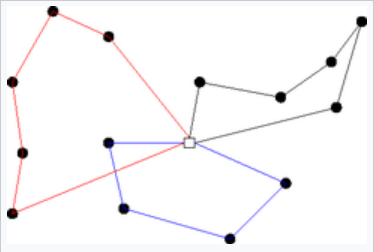
\includegraphics[scale=.45]{Graphics/vrp.png}
		\end{center}
		
		\caption{Representación del VRP: cada color representa la ruta de un vehículo y
		el cuadrado central, el almacén. Tomado de \cite{wiki}.\label{fig:vrp}}%
	\end{figure}

	El VRP y sus variantes se han estudiado durante más de 50 años \cite{Dantzig}.
	Algunas de estas son:

	\begin{itemize}
		\item \textit{Problema de Enrutamiento de Vehículos con Ventanas de Tiempo} 
			  (\textbf{VRPTW}, por sus siglas en inglés): Cada cliente tiene una ventana
			  de tiempo, o sea, un intervalo de tiempo en el cual el producto debe ser 
			  entregado.
	
		\item \textit{Problema de Enrutamiento de Vehículos Abierto} (\textbf{OVRP}, por
			  sus siglas en inglés): Las rutas de los vehículos no necesitan terminar en
			  el depósito.
	
		\item \textit{Problema de Enrutamiento de Vehículos con Res\-tric\-ción de Capacidad} 
			  (\textbf{CVRP}, por sus siglas en inglés): Los vehículos poseen capacidad 
			  limitada para llevar productos. El problema descrito anteriormente pertenece
			  a esta categoría.
	\end{itemize}

	El VRP es un problema NP-duro \cite{Paolo}, por lo que cualquier método exacto sólo es
	factible para instancias de pequeña dimensión. Estas características hacen de las 
	heurísticas y metaheurísticas grandes herramientas a tener en cuenta para resolverlos.

	Dentro de las metaheurísticas más usadas, destacan las de búsqueda local 
	\cite{Anand, Bianchi}: algoritmos basados en \textbf{criterios de vecindad}. Estos son 
	métodos en los que se define una solución actual, una estructura de entorno y de manera 
	iterativa se exploran las soluciones vecinas de la actual en busca de una nueva 
	solución. Las nuevas soluciones se aceptan o rechazan en dependencia de su calidad 
	para el problema y del algoritmo en cuestión. Por ejemplo, en \textit{Recocido Simulado} 
	se aceptan soluciones peores en base a determinada probabilidad que depende de un 
	parámetro del algoritmo \cite{Alina}.

	Dentro de las metaheurísticas de búsqueda local, la más usada es Búsqueda de Vecindad 
	Variable \cite{Mla}.
	
	La \textit{Búsqueda de Vecindad Variable} (\textbf{VNS}, por sus siglas en inglés) es un
	algoritmo de búsqueda local empleado para resolver instancias del CVRP, el cual utiliza 
	criterios de vecindad para obtener nuevas soluciones. Normalmente se utiliza una cantidad
	finita de criterios, sin embargo, en \cite{Camila} se propone una mo\-di\-fi\-ca\-ción 
	para considerar infinitos criterios, conocida como 
	\textit{Búsqueda de Vecindad Infinitamente Variable} (\textbf{IVNS}). En los experimentos 
	realizados en \cite{Camila} se obtuvieron buenos resultados. 
	
	Siguiendo la idea presentada en \cite{Camila}, en este trabajo se propone otra forma de 
	generar infinitos criterios de vecindad con el objetivo de comparar los resultados de 
	ambas vías.

	La estructura de este trabajo es: en la sección \ref{sec:nbhCrit} se definen los nuevos 
	criterios de vecindad y se presentan ejemplos. En la sección \ref{sec:impl} se explica 
	cómo se implementó la obtención de los criterios y el algoritmo IVNS. Los resultados se 
	exponen en la sección \ref{sec:res} y, por último, se presentan las conclusiones, 
	recomendaciones y trabajos futuros, en las secciones \ref{sec:conc} y \ref{sec:rec},
	respectivamente.

%===================================================================================



%===================================================================================
% Desarrollo
%-----------------------------------------------------------------------------------
\section{Criterios de Vecindad}\label{sec:nbhCrit}
%-----------------------------------------------------------------------------------

	En esta sección se explica qué es un criterio de vecindad y se presentan los 
	criterios de vecindad más usados para resolver el VRP.

  	Un \textit{criterio de vecindad} se define como una sucesión de operaciones, las
  	cuales son aplicadas a una solución para obtener otra, denominada \textit{vecina}
  	de la misma.

  	Todos los criterios de vecindad reportados en la literatura para solucionar el VRP,
  	\cite{Paolo, Alina} tienen un conjunto de operaciones en común \cite{Camila}, acciones elementales a 
  	partir de las cuales se pueden obtener los distintos criterios. Algunas de ellas son:
  	\begin{itemize}
  		\renewcommand{\labelitemi}{\tiny $\blacksquare$}
  		\item Seleccionar una ruta.
  		\item Seleccionar un cliente de una ruta.
  		\item Insertar un cliente en una ruta.
  		\item Eliminar un cliente de una ruta.
  	\end{itemize}

  	Estas operaciones se pueden clasificar en dos grupos disjuntos: \textbf{finales} y 
  	\textbf{no finales}.

	Las operaciones \textbf{finales} producen cambios en la solución, y cualquier 
	otra operación que pertenezca al criterio no depende de ella para ejecutarse. Las
	operaciones finales utilizadas en este trabajo son:
	
	\begin{itemize} % @todo actualizar las operaciones aleatorias q anyadimos
		\item Insertar cliente en una ruta (\textbf{b}).
		\item Intercambiar clientes de dos rutas (\textbf{c}).
		\item Insertar subruta en una ruta (\textbf{i}). % @audit esta letra ta mal. Revisa las dema's tambie'n
	\end{itemize}

	Las operaciones \textbf{no finales} son indispensables en la realización de otra
	operación. Las operaciones no finales utilizadas en este trabajo son:
	
	\begin{itemize}
		\item Seleccionar cliente de una ruta (\textbf{a}).
		\item Seleccionar ruta (\textbf{r}).
		\item Seleccionar subruta de una ruta (\textbf{s}).
	\end{itemize}

	Por ejemplo, para el criterio de vecindad \textit{insertar un cliente en una ruta},
	es necesario \textit{seleccionar una ruta} (\textbf{r}) y de ella \textit{seleccionar 
	un cliente} (\textbf{a}), para después \textit{seleccionar otra ruta} (\textbf{r}) 
	(o la misma) e \textit{insertar el cliente} en esta (\textbf{b}). Por ello se dice que 
	\textbf{b} depende de \textbf{r} y \textbf{a}, y este último, a su vez, depende de 
	\textbf{r}, de ahí que \textbf{r} y \textbf{a} sean operaciones no finales y \textbf{b} 
	sea final.
	
	Un criterio de vecindad se considera válido si cumple la regla siguiente:
	
	\begin{center}
		\fbox{
			\begin{minipage}{.45\textwidth}
				Posee al menos una operación final y cada o\-pe\-ra\-ción final tiene que 
				estar precedida, a la izquierda, por todas las operaciones no finales 
				de las cuales depende.
			\end{minipage}
			}
	\end{center}
	
	Si $\; V = \langle o_1, o_2, ..., o_n \rangle \;$ es un criterio de vecindad, donde
	$\; o_1, o_2, ..., o_n \;$ son operaciones, y se garantiza que en el momento de 
	ejecutar la operación $ o_i $, se hayan ejecutado previamente las operaciones 
	$\; o_j,\; 1 \leq \forall j < i $, entonces la regla asegura que se ejecuten 
	primero todas las operaciones de las cuales depende una operación final, 
	garantizando la correcta ejecución de esta.

	Por ejemplo, el criterio $\;rarac\;$ es válido, mientras que $\;rabr\;$ no lo es, 
	en este último la operación \textbf{r}, es una operación no final de la cual \textbf{b} 
	depende, pero \textbf{b} se encuentra a la izquierda de \textbf{r}, violando así la 
	regla anteriormente mencionada.

	Se define un \textit{criterio de vecindad simple} (\textbf{CVS}) como aquel que 
	contiene una y sólo una operación final. Ejemplos de CVS válidos son:
	\textit{rarb}, \textit{rarac} y \textit{raac}, descritos como \textit{insertar 
	cliente en una ruta}, \textit{intercambiar dos clientes de dos rutas} e
	\textit{intercambiar dos clientes de la misma ruta}, respectivamente.\\
	De esta manera, un criterio de vecindad es una sucesión, finita o no, de criterios 
	de vecindad simple.

	Hasta aquí se han definido cómo se formarán los criterios de vecindad y qu\'e
	características deben cumplir para considerarse válidos. A continuación se brindan 
	detalles sobre la implementación del algoritmo IVNS.
%-----------------------------------------------------------------------------------
\section{Implementación}\label{sec:impl}
%-----------------------------------------------------------------------------------
	En esta sección se presentan las ideas principales que se tuvieron en cuenta para 
	implementar la obtención de los infinitos criterios de vecindad y se hace una 
	des\-crip\-ción del algoritmo de búsqueda local.

	En lenguaje \textsc{C\#} se creó una jerarquía de clases para representar las 
	operaciones, la cual se muestra en la figura \ref{fig:hierarchy}; de esta forma,
	la adición de una operación no perjudica el buen funcionamiento del algoritmo.

	\begin{figure}[htb] % @todo actualizar esto con los comandos aleatorios
		\begin{center}
			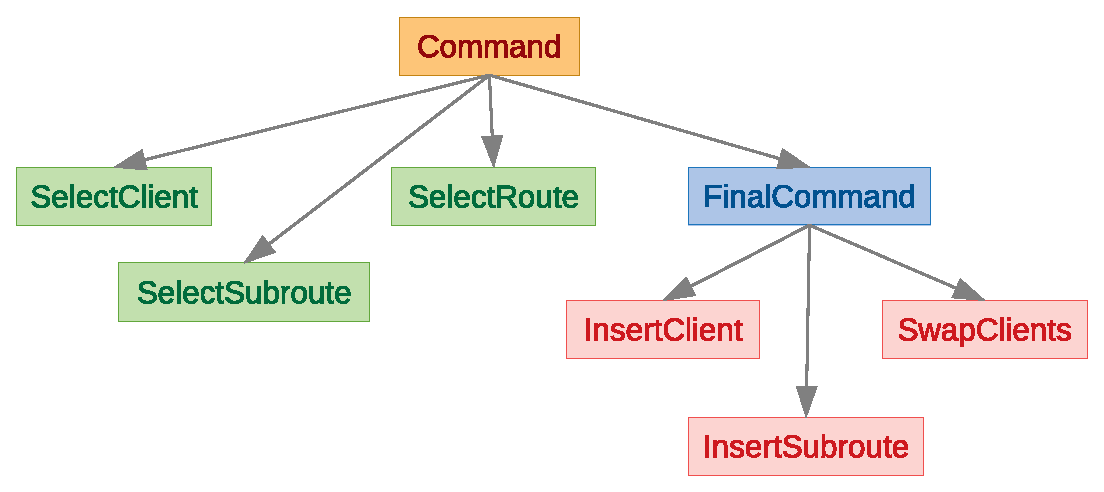
\includegraphics[scale=.43]{Graphics/hierarchy.eps}
		\end{center}
		\caption{Jerarquía de clases utilizada para representar a las operaciones.
		\label{fig:hierarchy}}
	\end{figure}
	
	Así, para añadir una operación, si esta es final, se crea una clase que herede de 
	\textsc{FinalCommand}, y si es no final, se crea una clase que herede directamente
	de \textsc{Command}.

	Si se quiere implementar IVNS, es necesario crear un método que sea capaz de generar 
	\textbf{infinitos criterios de vecindad}. Si se tiene un criterio 
	$V = \langle v_1, v_2, ..., v_n \rangle$, donde $\; v_1, v_2, ..., v_n \;$ son CVS,
	se puede crear un criterio distinto $V' = \langle v_1, v_2, ..., v_n, w \rangle$, 
	añadiéndole al final un CVS $w$ cualquiera. 
	
	Por ejemplo, si	$V = \langle rarac,\; rarb, \; rsri \rangle $, entonces $V'$ puede ser el 
	resultado de añadir el CVS $\;raac\;$ a $V$, de forma tal que 
	$V'= \langle rarac,\; rarb,\; rsri,\; raac \rangle$. De esta manera obtenemos infinitos 
	criterios de vecindad.
	
	A este enfoque para generar infinitos criterios se llamará 
	\textit{Generación de Criterios de Forma Creciente} o \textbf{SAG} (siglas en inglés para 
	\textit{Snake Approach Generator}), debido a que los criterios generados
	``crecen'', de forma similar a como lo hace la serpiente en el clásico videojuego 
	\textit{Snake}.

	La variante que se propone en este trabajo para IVNS se describe en el pseudocódigo 
	\ref{algor:IVNS} y utiliza la estrategia de \textbf{exploración exhaustiva}.

	Esta estrategia consiste en explorar todos los vecinos de la vecindad y devolver el 
	mejor de todos, para ello, se analizan todos los vecinos de la solución actual con
	respecto a todos los criterios $V$ compuestos por $n$ CVS, y se devuelve el mejor. La solución actual es inicialmente $S_0$ y se actualiza cada vez que se encuentra una soluci\'on mejor. $n$ es al comienzo igual a 1 y aumenta cuando no se encontr\'o una solución mejor o vuelve a ser 1, en caso contrario. Los criterios de vecindad son obtenidos mediante todas las combinaciones posibles de $n$ CVS, empleando para ello SAG. Se considera que una soluci\'on con costo $d_1$ es mejor que una soluci\'on con costo $d_2$ si $d_2 - d_1 > 10^{-3}$. La b\'usqueda de la mejor soluci\'on por todos los criterios de tamaño $n$ se detiene luego de $t_d$ milisegundos, mientras que todo el algoritmo se detiene luego de $ T $ milisegundos.

	\begin{algorithm}[htb]
		\caption{Snake IVNS} \label{algor:IVNS}
	
		\SetAlgoLined
	
		\KwData{$S_0, \;T, \; t_d$}
		\KwResult{Mejor solución encontrada.}
	
		\LinesNumbered
		\SetAlgoVlined
	
		iniciar un cron\'ometro para $ T $\;
		$best \leftarrow S_0$\;
		$ n \la 1 $\;
		\While{no se haya agotado $ T $}{
			reiniciar el cron\'ometro de $ t_d $\;
			\ForEach{criterio $ V $ compuesto por $ n $ CVS}{
				\If{se agot\'o $ T $ o $ t_d $}{
					\textbf{break}\;
				}
				$x \la $ mejor vecino de $best$ en $ V $\;
				\If{x es mejor que best}{
					$x \la best$\;
				}
			}
			\If{mejor\'o $ best $}{
				$ n \la 0 $\;
			}
			$ n \la n + 1 $\;
		}
		\Return $best$\;
		
	\end{algorithm}
	
	Hasta aquí se presentó el algoritmo utilizado para generar los infinitos criterios 
	y se describió la estrategia de exploración utilizada. En la sección siguiente se
	presentan los resultados obtenidos por este algoritmo y se comparan con los resultados
	obtenidos al aplicar el algoritmo descrito en \cite{Camila}. Ambos se aplicaron para 
	resolver las mismas instancias del CVRP. Estas instancias se obtuvieron de \cite{neo}.
	
%-----------------------------------------------------------------------------------
\section{Resultados}\label{sec:res}
%-----------------------------------------------------------------------------------
	En este apartado se muestra el desempeño del algoritmo presentado en este artículo
	(Snake IVNS) y se compara con el mejor resultado obtenido por el IVNS presentado en 
	\cite{Camila}, al resolver los problemas \textbf{A-n33-k5}, \textbf{A-n34-k5}, 
	\textbf{A-n36-k5}, \textbf{A-n65-k9} y \textbf{A-n80-k10}, extraídos de \cite{neo}.

	En la figura \ref{fig:results} se muestran los costos de la mejor soluci\'on reportada por \cite{benchmark}, \cite{Camila} y la encontrada por el algoritmo descrito en este art\'iculo. Snake IVNS fue ejecutado 30 veces en cada problema y en cada una de ellas se tom\'o $T = 30000, t_d = 5000$ y a $S_0$ como el resultado de repartir aleatoriamente a los clientes en rutas, satisfaciendo las condiciones del problema.

	\begin{figure}[h!]%
		\begin{center}
			\begin{tabular}{|c|c|c|c|} \hline
			Problema 	& \cite{benchmark} & \cite{Camila} & Snake \\ \hline
			A-n33-k5 			&  	661		&  \textbf{640}		& 662 \\ \hline
			A-n34-k5 & 778 & \textbf{737} & 789 \\ \hline
			A-n36-k5 & \textbf{799} & 805 & 818 \\ \hline
			A-n65-k9			& 	\textbf{1174}		& 1311		& 1253	\\ \hline
			A-n80-k10 			& 	\textbf{1764}		&  	2069	& 1903	\\ \hline
			\end{tabular}
			\caption{Costo de la mejor soluci\'on. \label{fig:results}}
		\end{center}
	\end{figure}
	
	% En las figuras \ref{fig:result33_5}, \ref{fig:result34_5}, \ref{fig:result36_5},
	% \ref{fig:result65_9} y \ref{fig:result80_10}, se puede apreciar la solución de menor
	% costo que Snake IVNS encontró después de ser exploradas un número de 
	% soluciones, así como el costo mínimo reportado en \cite{neo} y el costo 
	% mínimo obtenido por	IVNS para cada uno de los problemas trabajados.

	Se puede apreciar c\'omo \cite{Camila} es mejor que \cite{benchmark} y que Snake en A-n33-k5 y A-n34-k5. Aunque \cite{Camila} no supera a \cite{benchmark} en A-n36-k5, s\'i lo hace con respecto a Snake. Esto no sucede de igual manera en los \'ultimos dos problemas, donde Snake alcanza una soluci\'on mejor que \cite{Camila}, aunque no mejor que \cite{benchmark}.

	Si tenemos en cuenta que cada corrida de Snake s\'olo dispuso de 30 segundos para alcanzar los resultados de la figura \ref{fig:results}, entonces se puede decir que el algoritmo tuvo un buen desempeño.

	A continuación se muestran, para cada problema, la distribución de 
	rutas que logra el mejor resultado obtenido en Snake IVNS. 
	En cada ruta se encuentran los identificadores de los clientes ubicados	en esa ruta. 
	Estos identificadores son números naturales del 1 al $n-1$, donde $n$ es la cantidad 
	de clientes del problema m\'as el almac\'en ($n = 33\;$ para A-n33-k5,
	$n = 34\;$ para A-n34-k5, $n = 36\;$ para A-n36-k5, etc).
	
	% % ----------------------- 33 5 ---------------------------------
	% \begin{figure}[htbp]
	% 	\centering
	% 	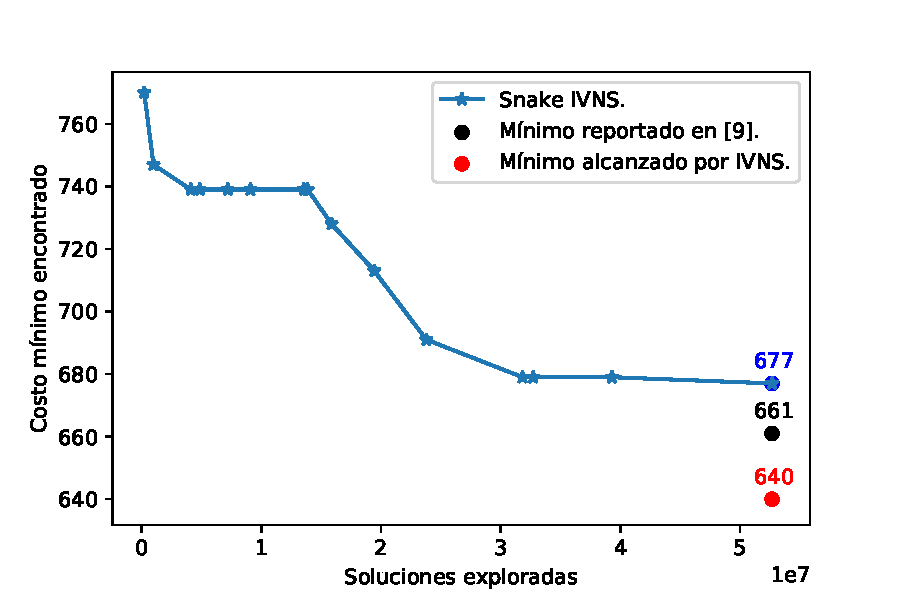
\includegraphics[scale=.55]{Graphics/result_A-n33-k5.pdf}
	% 	\caption{Desempeño del algoritmo en A-n33-k5.}\label{fig:result33_5}
	% \end{figure}
	% % --------------------------- 34 5 ----------------------------------
	% \begin{figure}[ht]
	% 	\centering
	% 	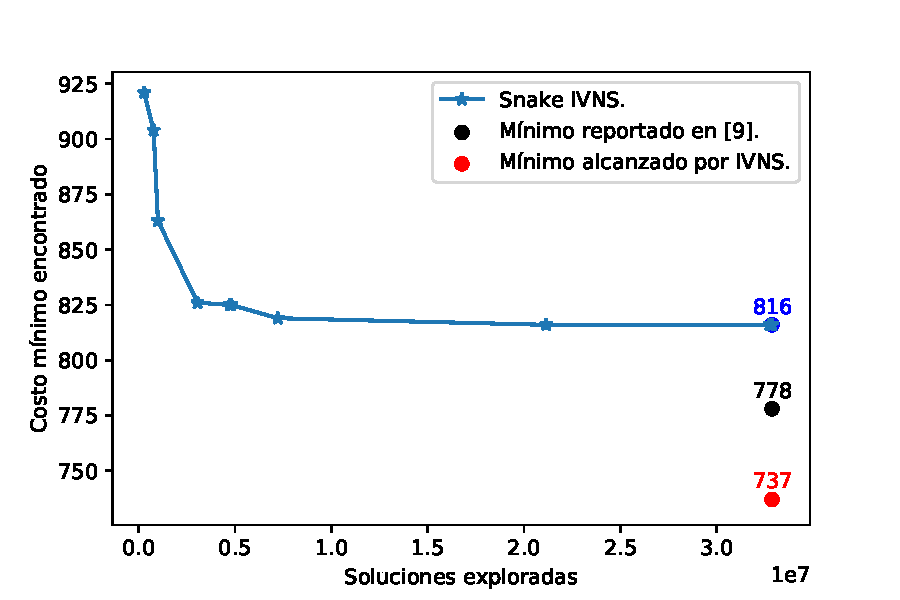
\includegraphics[scale=.55]{Graphics/result_A-n34-k5.pdf}
	% 	\caption{Desempeño del algoritmo en A-n34-k5.}\label{fig:result34_5}
	% \end{figure}
	
	% En las figuras \ref{fig:result33_5} y \ref{fig:result34_5} se aprecia cómo el 
	% algoritmo IVNS supera ampliamente a Snake IVNS y al mejor resultado presentado en 
	% \cite{neo}.
	
	% % --------------------------- 36 5 ----------------------------------
	% \begin{figure}[H]
	% 	\centering
	% 	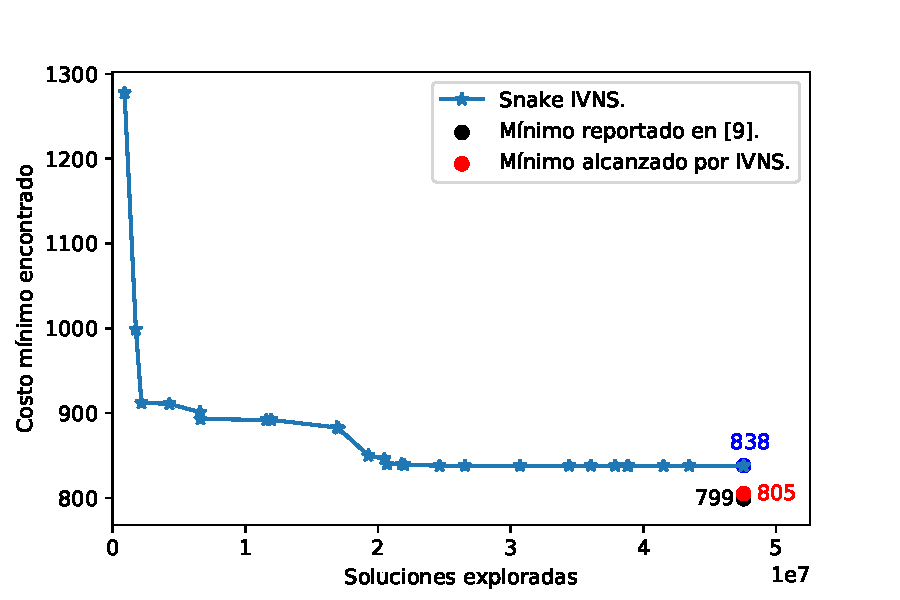
\includegraphics[scale=.55]{Graphics/result_A-n36-k5.pdf}
	% 	\caption{Desempeño del algoritmo en A-n36-k5.}\label{fig:result36_5}
	% \end{figure}
	
	% % -------------------------- 65 9 ------------------------------
	% \begin{figure}[htbp]
	% 	\centering
	% 	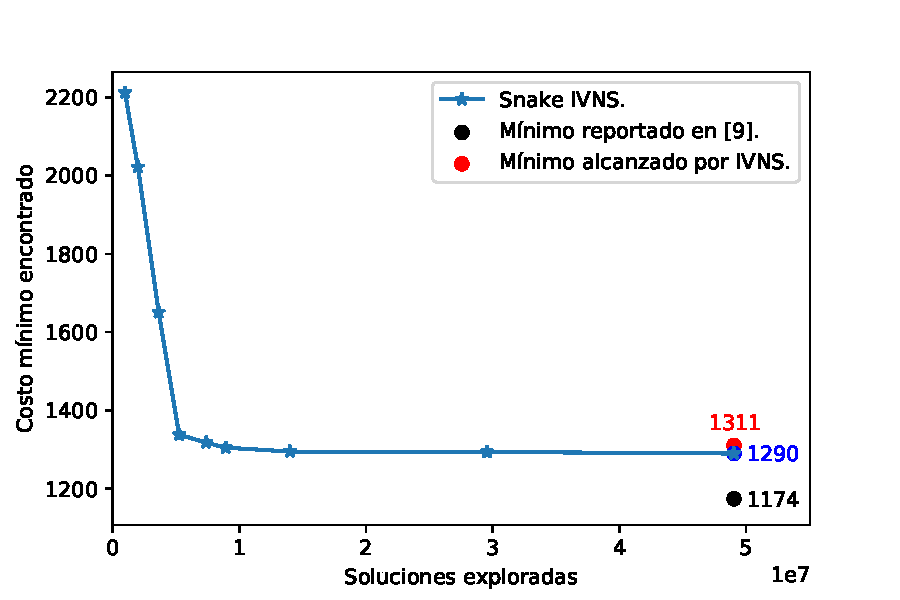
\includegraphics[scale=.55]{Graphics/result_A-n65-k9.pdf}
	% 	\caption{Desempeño del algoritmo en A-n65-k9.}\label{fig:result65_9}
	% \end{figure}
	
	% % ---------------------------- 80 10 ---------------------------------
	% \begin{figure}[H]
	% 	\centering
	% 	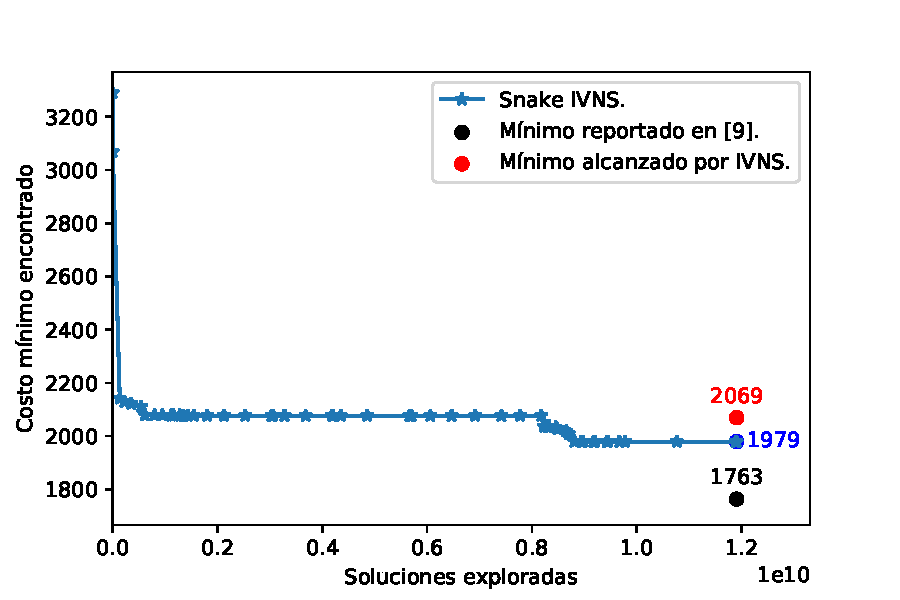
\includegraphics[scale=.55]{Graphics/result_A-n80-k10.pdf}
	% 	\caption{Desempeño del algoritmo en A-n80-k10.}\label{fig:result80_10}
	% \end{figure}
	
	% En la figura \ref{fig:result36_5} se puede apreciar cómo IVNS no mejora el
	% mínimo presentado en \cite{neo}, pero sigue obteniendo un mejor resultado que 
	% Snake IVNS. Sin embargo, en las figuras \ref{fig:result65_9} y \ref{fig:result80_10},
	% Snake IVNS consigue ser mejor que IVNS. Todo parece indicar que el algoritmo presentado
	% en \cite{Camila} disminuye su rendimiento cuando aumenta la cantidad de clientes,
	% mientras que Snake IVNS se mantiene estable en su ejecución.

	\section*{Distribución de rutas para el problema A-n33-k5.}
	\label{tab:result33_5}

	% \hspace{9pt} \textbf{Usando \blue{Snake IVNS}}\\				  
	\hspace{-10pt}\textbf{Ruta 1:} 23, 18, 28, 22 \\
	\textbf{Ruta 2:} 11, 31, 1, 21, 14, 19, 6, 24 \\
	\textbf{Ruta 3:} 20, 4, 27, 25, 30, 10 \\
	\textbf{Ruta 4:} 29, 16, 3, 9, 17, 15 \\
	\textbf{Ruta 5:} 12, 5, 26, 7, 8, 13, 32, 2 \\

	% \textbf{Usando \red{IVNS}} 							\\
	% \textbf{Ruta 1:} 11, 18, 28, 23 					\\
	% \textbf{Ruta 2:} 2, 4, 12, 5, 27, 25, 30, 10, 17, 9 \\
	% \textbf{Ruta 3:} 32, 13, 8, 7, 26, 20 				\\
	% \textbf{Ruta 4:} 24, 6, 19, 14, 21, 1, 31 			\\
	% \textbf{Ruta 5:} 29, 3, 16, 15, 22 					
	
	\section*{Distribución de rutas para el problema A-n34-k5.}
	\label{tab:result34_5}
	
	% \hspace{9pt} \textbf{Usando \blue{Snake IVNS}}
	\hspace{-10pt}\textbf{Ruta 1:} 24, 30, 5, 26, 4 \\
	\textbf{Ruta 2:} 14, 8, 15, 6, 7, 10 \\
	\textbf{Ruta 3:} 18, 21, 32, 28, 31, 25, 13 \\
	\textbf{Ruta 4:} 20, 33, 16, 22, 3, 12, 9, 2 \\
	\textbf{Ruta 5:} 17, 19, 11, 23, 27, 1, 29 \\

	% \textbf{Usando \red{IVNS}}						\\
	% \textbf{Ruta 1:} 18, 16, 22, 12, 3, 9, 2 		\\
	% \textbf{Ruta 2:} 20, 33, 4, 26 					\\
	% \textbf{Ruta 3:} 10, 13, 7, 6, 15, 8, 14		\\
	% \textbf{Ruta 4:} 21, 32, 28, 25, 31, 17, 19, 11 \\
	% \textbf{Ruta 5:} 5, 30, 24, 27, 23, 1, 29		
	
	\section*{Distribución de rutas para el problema A-n36-k5.}
	\label{tab:result36_5}
	
	% \hspace{9pt} \textbf{Usando \blue{Snake IVNS}}
	\hspace{-10pt}\textbf{Ruta 1:} 24, 21, 22, 32, 18, 30, 17, 13, 1, 16	\\
	\textbf{Ruta 2:} 10, 7	\\
	\textbf{Ruta 3:} 27, 33, 29, 31, 19, 4, 6, 3, 12	\\
	\textbf{Ruta 4:} 15, 8, 35, 2, 23, 34, 14, 28	\\
	\textbf{Ruta 5:} 26, 20, 5, 9, 25, 11 \\
	
	% \textbf{Usando \red{IVNS}}						 \\
	% \textbf{Ruta 1:} 16, 1, 22, 32, 24, 27, 25, 11   \\
	% \textbf{Ruta 2:} 20, 14, 34, 6, 3, 4, 19, 31, 12 \\
	% \textbf{Ruta 3:} 5, 9, 28, 23, 2, 35, 8, 15, 7   \\
	% \textbf{Ruta 4:} 26, 10						     \\
	% \textbf{Ruta 5:} 21, 18, 33, 29, 30, 17, 13	     
	
	\section*{Distribución de rutas para el problema A-n65-k9.}
	\label{tab:result65_9}
	
	% \hspace{9pt} \textbf{Usando \blue{Snake IVNS}}		 \\
	\hspace{-10pt}\textbf{Ruta 1:} 3, 36, 50, 16, 2, 41 \\
	\textbf{Ruta 2:} 34, 31, 26, 6, 64, 46, 47 \\
	\textbf{Ruta 3:} 62, 33, 1, 12, 13, 29 \\
	\textbf{Ruta 4:} 28, 23, 57, 48, 54, 63, 11, 7 \\
	\textbf{Ruta 5:} 21, 59, 44, 56, 25, 18 \\
	\textbf{Ruta 6:} 43, 27, 14, 9, 22, 15 \\
	\textbf{Ruta 7:} 55, 40, 10, 8, 52, 24, 19 \\
	\textbf{Ruta 8:} 60, 30, 37, 35, 4, 49 \\
	\textbf{Ruta 9:} 53, 32, 20, 58, 61, 42, 38, 45, 5 \\
	\textbf{Ruta 10:} 17, 51, 39\\ 
	
	% \textbf{Usando \red{IVNS}}						   \\
	% \textbf{Ruta 1:} 17, 15, 22, 9, 14, 27, 43		   \\
	% \textbf{Ruta 2:} 40, 10, 8, 52, 24, 19, 25		   \\
	% \textbf{Ruta 3:} 32, 20, 58, 61, 42, 45, 5		   \\
	% \textbf{Ruta 4:} 57, 48, 54, 11, 7				   \\
	% \textbf{Ruta 5:} 4, 3, 36, 35, 37				   \\
	% \textbf{Ruta 6:} 49, 30, 60, 50, 16, 2, 38, 41	   \\
	% \textbf{Ruta 7:} 55, 29, 18, 13, 12, 1, 33, 23, 28 \\
	% \textbf{Ruta 8:} 47, 34, 31, 26, 6, 46, 39, 51	   \\
	% \textbf{Ruta 9:} 53, 59, 56, 44, 21			       \\
	% \textbf{Ruta 10:} 62, 63, 64					   
	
	\section*{Distribución de rutas para el problema A-n80-k10.}
	\label{tab:result80_10}
	
	% \hspace{9pt} \textbf{Usando \blue{Snake IVNS}}											\\
	\hspace{-10pt}\textbf{Ruta 1:} 10, 71, 52, 2, 37, 8, 6	\\
	\textbf{Ruta 2:} 53, 76, 50, 45, 22, 4, 32	\\
	\textbf{Ruta 3:} 17, 20, 75, 19, 57, 61	\\
	\textbf{Ruta 4:} 72, 54, 9, 55, 41, 25, 46, 31, 74	\\
	\textbf{Ruta 5:} 28, 79, 18, 48, 14, 21	\\
	\textbf{Ruta 6:} 30, 78, 68, 16, 43, 26, 65, 35, 69, 56, 47, 15, 33, 64, 60, 39, 77	\\
	\textbf{Ruta 7:} 12, 44, 5, 23, 62, 7	\\
	\textbf{Ruta 8:} 42, 51, 3, 1, 40	\\
	\textbf{Ruta 9:} 49, 38, 58, 70, 66, 67, 36, 73 \\
	\textbf{Ruta 10:} 63, 11, 34, 24, 59, 27, 29, 13	\\
	
	% \textbf{Usando \red{IVNS}}								\\
	% \textbf{Ruta 1:} 49, 38, 32, 4, 22, 45, 50, 72, 76, 73	\\
	% \textbf{Ruta 2:} 53, 39, 60, 3, 77, 42		   			\\
	% \textbf{Ruta 3:} 7, 21, 40		   						\\
	% \textbf{Ruta 4:} 1, 63, 11, 52, 28, 18, 48, 14, 71, 10	\\
	% \textbf{Ruta 5:} 64, 15, 56, 47, 20, 31, 17, 74		    \\
	% \textbf{Ruta 6:} 62, 34, 2, 37, 8, 30, 5	   			\\
	% \textbf{Ruta 7:} 12, 44, 6, 24, 23, 13 					\\
	% \textbf{Ruta 8:} 78, 68, 43, 16, 61, 57, 75, 27, 29	    \\
	% \textbf{Ruta 9:} 36, 67, 66, 58, 33, 41, 25, 46, 51		\\
	% \textbf{Ruta 10:} 59, 19, 26, 65, 35, 69, 55, 9, 54, 70	\\
	% \textbf{Ruta 11:} 79									\\
	
	% @remind comparar esto d las rutas (si las pones junto con las d cami)

	En esta sección se pudo observar el desempeño de los algoritmos de tipo IVNS y
	los buenos resultados que se pueden alcanzar al considerar infinitos criterios
	de vecindad. En las secciones siguientes se presentan las conclusiones del trabajo
	y las recomendaciones y trabajos futuros.
	
%===================================================================================

%===================================================================================
% Conclusiones
%-----------------------------------------------------------------------------------
\section{Conclusiones}\label{sec:conc}

  El problema de enrutamiento de vehículos es uno de los problemas de gestión más
  comunes en la distribución de alimentos y combustible. Para resolver una de sus
  variantes, CVRP, se presentó en este trabajo una metaheurística del tipo Búsqueda 
  de Vecindad Infinitamente Variable.
  
  Se pudo apreciar cómo considerar infinitos criterios de vecindad no es una idea
  descabellada, al observar los buenos resultados que obtienen los algoritmos de este
  tipo, particularmente, el presentado en este artículo.

%===================================================================================



%===================================================================================
% Recomendaciones
%-----------------------------------------------------------------------------------
\section{Recomendaciones}\label{sec:rec}

  Como recomendación, se propone implementar el algoritmo, así como la jerarquía de
  clases, en lenguaje \textsc{C++}, para reducir los costos propios del lenguaje
  y así mejorar la eficiencia del proyecto. Se recomienda, también, implementar una
  estructura de datos que permita la realización de las operaciones sobre una ruta
  eficientemente, para de esta forma disminuir el costo computacional para instancias
  del problema con grandes cantidades de clientes.
  
  Los trabajos futuros se deben orientar en este sentido, aumentando la experimentación
  para obtener resultados más palpables.
  
%===================================================================================



%===================================================================================
% Bibliografía
%-----------------------------------------------------------------------------------
\begin{thebibliography}{99}
%-----------------------------------------------------------------------------------
	\bibitem{Camila} Pérez Mosquera, C. (2017).	\emph{Primeras aproximaciones 
	a la Búsqueda de Vecindad Infinitamente Variable}. Facultad de Matemática y Computación, 
	Universidad de La Habana.
	
	\bibitem{Paolo} Paolo Toth; Daniele Vigo (2001) $\;$ \textit{The Vehicle Routing 
	Problem (Monographs on Discrete Mathematics and Applications)}. Monographs on 
	Discrete Mathematics and Applications. SIAM $\;$
	MIT Press.
	
	\bibitem{Dantzig} J. H. Dantzig, G. B.; Ramser. $\;$\textit{The truck dispatching 
	problem. volume 6.} $\;$ INFORMS, 10 1959.
	
	\bibitem{Anand} Anand; Ochi Luiz Satoru Penna, Puca Huachi Vaz; Subramanian.$\;$ 
	\textit{An iterated local search heuristic for the heterogeneous fleet vehicle 
	routing problem}. $\;$ Journal of Heuristics, 19, 04 2013.

	\bibitem{Bianchi} Leonora Bianchi; Ann Melissa Campbell. $\;$ \textit{Extension of 
	the 2-p-opt and 1-shift algorithms to the heterogeneous probabilistic traveling 
	salesman problem}.$\;$ European Journal of Operational Research, 176, 2007.

	\bibitem{Alina}  Alina Fernández Arias. $\;$ \textit{El problema de enrutamiento de 
	vehículos con recogida y entrega simultánea considerando una flota heterogénea.} 
	$\;$ Master’s thesis, Facultad de Matemática y Computación. Universidad de La Habana, 
	La Habana, Cuba, 7 2010.
	
	\bibitem{Mla} N Mladenovic. $\;$ \textit{A variable neighborhood algorithm - a new 
	metaheuristic for optimization combinatorial.}$\;$ In Abstract of papers presented at 
	Optimization Days, Montreal, volume 12, 1995.

	\bibitem{wiki} \textit{Wikipedia}.\\
	URL: \href{https://en.wikipedia.org/wiki/Vehicle\_ routing\_ problem}
	{https://en.wikipedia.org/wiki/Vehicle\_ routing\_ problem}
	
	\bibitem{neo} \textit{NEO Networking and Emerging Optimization.	Instancias de pruebas
	para vrp.} \\
	URL: \href{http://neo.lcc.uma.es/vrp/vrpinstances/capacitated-vrp-instances/}
	{http://neo.lcc.uma.es/vrp/vrpinstances/capacitated-vrp-instances/}, 1 2013.

	\bibitem{benchmark} Surana, Pratik, \textit{Benchmarking Optimization Algorithms for Capacitated Vehicle Routing Problems} (2019). Master's Projects. 719.
	DOI: \href{https://doi.org/10.31979/etd.cjjg-7wvf}{https://doi.org/10.31979/etd.cjjg-7wvf}.
	\href{https://scholarworks.sjsu.edu/etd\_projects/719}{https://scholarworks.sjsu.edu/etd\_projects/719}
%-----------------------------------------------------------------------------------
\end{thebibliography}

%-----------------------------------------------------------------------------------

\label{end}

\end{document}

%===================================================================================
